\chapter{Исследовательская часть}
В этом разделе будет продемонстрирована работа программы, а также
приведены результаты тестирования алгоритмов.

\section{Демонстрация работы программы}
На рисунках 4.1-4.2 приведена демонстрация работы программы для линейной реализации алгоритма и параллельной.

\FloatBarrier
\begin{figure}[h]
	\begin{center}
		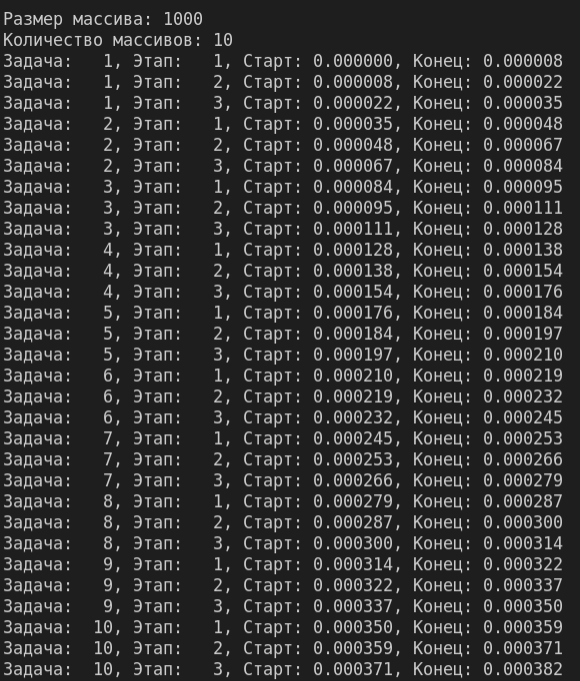
\includegraphics[]{inc/linear.png}
	\end{center}
	\caption{Демонстрация работы линейного алгоритма}
\end{figure}
\FloatBarrier

\FloatBarrier
\begin{figure}[h]
	\begin{center}
		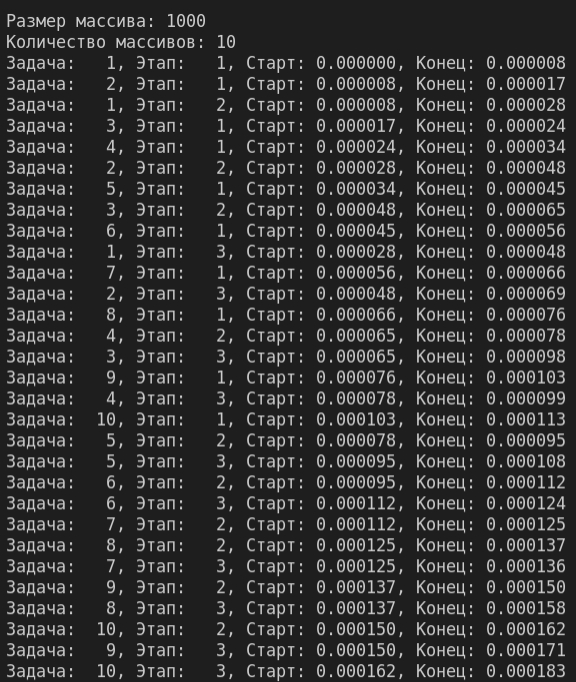
\includegraphics[]{inc/paral.png}
	\end{center}
	\caption{Демонстрация реализации за счёт вычислительного конвейера}
\end{figure}
\FloatBarrier

\section{Технические характеристики}
Технические характеристики устройства, на котором выполнялось тестирование, следующие:
\begin{itemize}
	\item операционная система: Ubuntu 20.04.1 LTS;
	\item память: 8 GB;
	\item процессор: Intel Core i5-1135G7 @ 2.40GHz \cite{intel}.
	\item количество ядер процессора: 8
\end{itemize}

Во время тестирования ноутбук был нагружен только встроенными приложениями окружения, а также непосредственно системой тестирования.

\section{Тестирование программы}
Тестирование будет производиться для двух различных ситуаций.

В первом случае во всех массивах 5000 элементов, и тестирование будет производиться на разном количестве массивов.
Во втором случае будет зафиксировано 50 массивов, и тестирование будет производиться на разном числе элементов в массиве.

Это сделано для того, чтобы можно было сделать более подробный вывод насчёт конвейерных вычислений.

Результаты тестирования первого случая представлены в таблице (время - в мс). 
В первом столбце - размер массива, во втором - время работы линейного конвейера, в третьем - параллельного.

\FloatBarrier
\begin{table}[h]
	\caption{Результаты тестов}
	\centering
	\begin{tabular}{ | l | l | l |}
		\hline
		Размер массива & Линейный & Параллельный\\ 
		\hline
		2 & 0.000339 & 0.000234\\
		5 & 0.000850 & 0.000547\\
		10 & 0.002557 & 0.001240\\
		25 & 0.002948 & 0.001512\\
		50 & 0.004570 & 0.001927\\
		75 & 0.009906 & 0.005649\\
		100 & 0.008375 & 0.003910\\
		150 & 0.012908 & 0.005777\\
		200 & 0.018446 & 0.010047\\
		300 & 0.027001 & 0.015216\\
		500 & 0.042561 & 0.020329\\
		700 & 0.081352 & 0.038265\\
		850 & 0.092877 & 0.032452 \\
		1000 & 0.094582 & 0.041348\\
		\hline
	\end{tabular}
\end{table}
\FloatBarrier

На рисунке 4.1 показан график зависимости времени работы алгоритмов от количества массивов.

\FloatBarrier
\begin{figure}[h]
	\begin{center}
		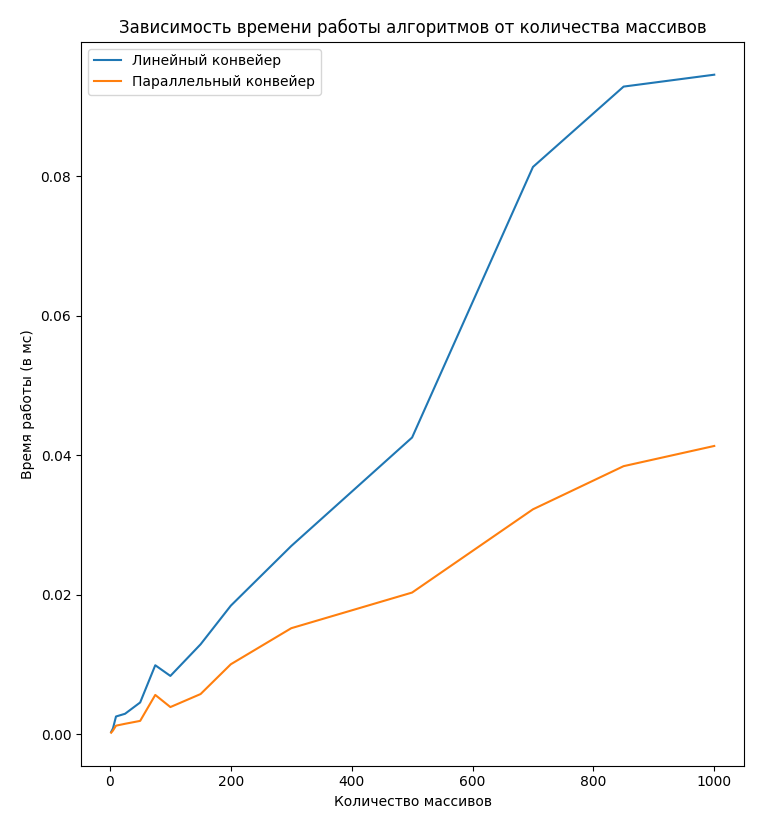
\includegraphics[width=\linewidth]{inc/number.png}
	\end{center}
	\caption{График зависимости времени работы алгоритмов от количества массивов}
\end{figure}
\FloatBarrier


Результаты тестирования второго случая представлены в таблице (время - в мс).
В первом столбце - размер массива, во втором - время работы линейного конвейера, в третьем - параллельного.

\FloatBarrier
\begin{table}[h]
	\caption{Результаты тестов}
	\centering
	\begin{tabular}{ | l | l | l |}
		\hline
		Количество элементов массива & Линейный & Параллельный\\ 
		\hline
		2 & 0.000179 & 0.000036\\
		5 & 0.000192 & 0.000066\\
		10 & 0.000371 & 0.000105\\
		50 & 0.000908 & 0.000185\\
		100 & 0.002483 & 0.000395\\
		200 & 0.003450 & 0.000996\\
		300 & 0.003985 & 0.001116\\
		500 & 0.005747 & 0.001290\\
		750 & 0.006763 & 0.002194\\
		1000 & 0.008604 & 0.003437\\
		2000 & 0.012041 & 0.007453\\
		3000 & 0.017266 & 0.012255\\
		5000 & 0.030266 & 0.018450\\
		6000 & 0.038714 & 0.018948\\
		7000 & 0.040697 & 0.021442\\
		8000 & 0.052930 & 0.027142\\
		10000 & 0.072837 & 0.031553\\
		\hline
	\end{tabular}
\end{table}
\FloatBarrier

На рисунке 4.1 показан график зависимости времени работы алгоритмов от размера массивов.

\FloatBarrier
\begin{figure}[h]
	\begin{center}
		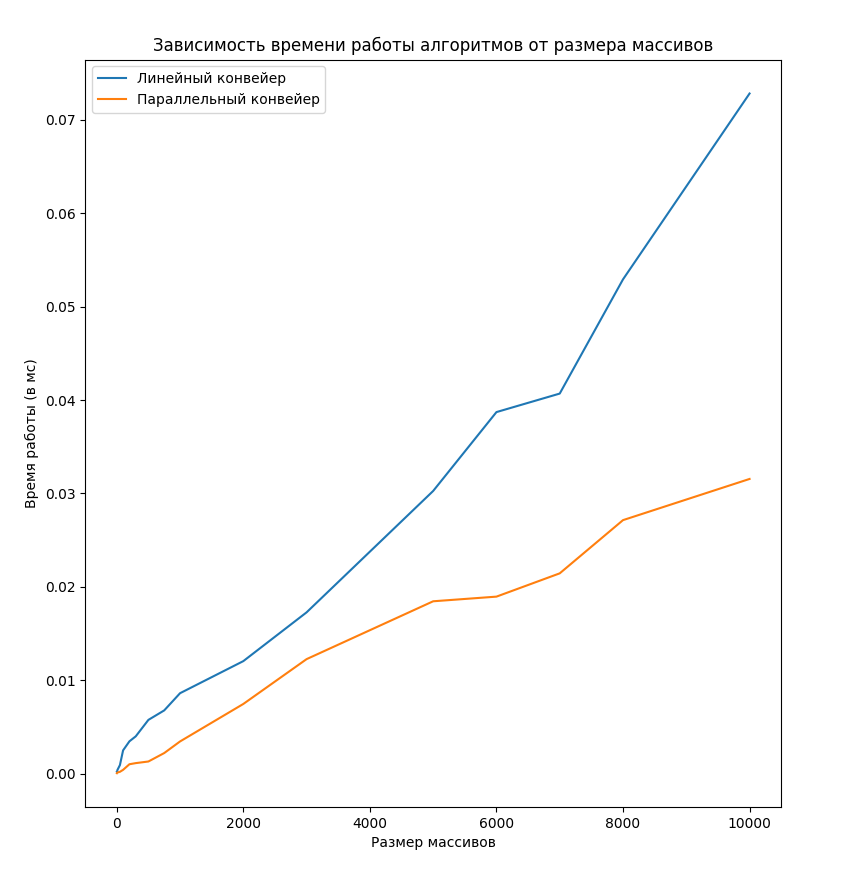
\includegraphics[width=\linewidth]{inc/size.png}
	\end{center}
	\caption{График зависимости времени работы алгоритмов от размера массивов}
\end{figure}
\FloatBarrier

\section{Вывод}
Параллельный конвейер оказался более быстрым по всем измерениям. 
При количестве массивов $ N = 10 $ параллельный алгоритм работает в 2.06 раз быстрее, чем линейная реализация.
При количестве массивов $ N = 700 $ параллельная реализация опередила линейную в 2.12 раз, а на 
$ N = 1000 $ разница достигла 2.3 раз.
Уже при размере очереди в два элемента реализация вычислительного конвейера оправдывает себя.

При фиксированном количестве массивов (500) параллельный конвейер также быстрее при любом размере массива.
При размере массива $ N = 50 $ параллельная реализация опередила линейную в 5.34 раза. 
При $ N = 5000 $ конвейер был быстрее в 1.6 раз, при $ N = 10000 $ --  в 2.3 раза.

Таким образом, конвейер позволил существенно увеличить скорость выполнения задачи, разделив 
одну задачу на несколько простых.